\documentclass[11pt]{article}
\usepackage{freerbmt09}

\usepackage[pdftex]{graphicx}
%\usepackage{graphics}
%\usepackage{rotating}
%\usepackage{ucs}

\usepackage[utf8x]{inputenc}
\usepackage{times}
\usepackage{natbib}
\usepackage{url}
\usepackage{latexsym}

%\usepackage{tabularx}
\usepackage[small,bf]{caption}

%%\newtheorem{cs}{Case Study}


\title{Implementing an efficient and scalable service-oriented architecture for the Apertium machine translation platform}

\author{Pasquale Minervini\\
  Dipartimento di Informatica\\
  Università degli Studi di Bari\\
  Via E. Orabona 4, 70125 Bari, Italy\\
  {\tt p.minervini@gmail.com}}

\date{}

\begin{document}

\maketitle

\begin{abstract}
Service Oriented Architecture (SOA) is a paradigm for organising and using distributed services that may be under the control of different ownership domains and implemented using various technology stacks. In some contexts, an organisation using an IT infrastructure implementing the SOA paradigm can take a great benefit from the integration, in its business processes, of efficient machine translation (MT) services to overcome language barriers. This paper describes the architecture and the design patterns used to develop an MT service that is efficient, scalable and easy to integrate in new and existing business processes. The service is based on Apertium, a free/open-source rule-based machine translation platform.
\end{abstract}


\section{Introduction}

Service Oriented Architecture is an architectural paradigm providing a set of principles of governing concepts used during phases of systems development and integration. In such an architecture, functionalities are packaged as interoperable, loosely coupled services that may be used to build infrastructures enabling those with needs (consumers) and those with capabilities (providers) to interact across different domains of technology and ownership.

Several new trends in the computer industry rely upon SOA as their enabling foundation, including the automation of Business Process Management (BPM) and the multitude of new architecture and design patterns generally referred to as Web~2.0~\citep{web20}.

In some contexts, an organisation using an IT infrastructure implementing the SOA paradigm can take a great benefit from the integration, in its business processes, of an efficient machine translation service to overcome language barriers; for instance, it could be integrated in collaborative enviroments where people, who have no language in common, attempt to communicate with each other, or in knowledge extraction processes, where data is not available in a language that can be understood by the domain experts or the knowledge extraction tools being used.

A machine translation service was creating using Apertium\footnote{\url{http://www.apertium.org/}}~\citep{armentano05p}, a free/open-source rule-based machine translation platform for its translation capabilities, and on libTextCat\footnote{\url{http://software.wise-guys.nl/libtextcat/}}, a library implementing n-gram based text categorisation~\citep{textcat} for language recognition, which provides an inexpensive and highly effective way of recognising the language used in documents; this result is reached by using small-sized (about $4KB$) fingerprints of the desired languages rather than resorting to more complicated and costly methods such as natural language parsing or assembling detailed lexicons. The libTextCat library is also used by Bitextor~\citep{espla-gomis2009bfs}, a system to harvest translation memories from multilingual websites.

%% REVIEWER #1: "In section 1, authors claim that their system includes 
%%   a language detector, but there is no later mention to it in the 
%%   paper." What is the error rate of the new system? 
%%           Where is it used? 
%%           Have experiments been conducted on it?
%%
%%  DESCRIBE WHY TEXTCAT WAS USED (IT IS THE BEST -- GIVE SOME NUMBERS ETC.) -FMT


%Our decision to prefer a rule-based
%machine translation system to a statistical or an example-based machine translation system was 
%motivated by the following reasons:

%\begin{itemize}
% \item 
% \item Statistical Machine Translation systems tend to produce text that appears more ``natural'' than that produced by Rule-Based ones, with the result that ``fluency'' can outweight ``fidelity'', but a natural and fluent translation is not necessairly completely faithful to the original text;
% \item In Rule-Based Machine Translation systems, linguistic knowledge can be encoded explicitly in the form of linguistic data, so that both humans and automatic systems can process it (this feature can be a great benefit when using domain-specific linguistic knowledge);
% \item Rule-Based Machine Translation systems tend to produce more ``mechanical'' translations, so their errors tend also to be more evident;
% \item Experts who have designed a Rule-Based Machine Translation system find it much easier to diagnose and repair sources of translation errors, like wrong rules in modules or wrong entries in dictionaries.
%\end{itemize}

Efficiency and scalability are critical for the service since, especially in collaborative enviroments, it should be able to sustain a heavy load of traffic. In this paper, the techniques and design patterns used to implement the machine translation service will be described and it will be compared to the standalone system.

%% You should probably put some note about the alternative (Víctor's service here) p.2 of his paper

\section{Service APIs}

Our service provides the two following capabilities:

\begin{itemize}
  \item Translation -- for automatic translation of free text from a source language to a destination language;
  \item Language recognition -- for automatic language guessing of free text;
\end{itemize}

In SOA, interoperability between services is achieved by using standard languages for the description of service interfaces and the communications among services. A widely accepted technique for implementing SOA consists in making use of Web Services~\citep{soa}; a Web  Service is defined by the W3C as ``a software system designed to support interoperable machine-to-machine interaction over a network. It has an interface described in a machine-processable format (specifically WSDL). Other systems interact with the Web service in a manner prescribed by its description using SOAP-messages, typically conveyed using HTTP with an XML serialization in conjunction with other Web-related standards.''~\citep{wsgloss}. 

Alternative standards to SOAP are XML-RPC~\citep{xmlrpcspec}, a remote procedure call protocol which uses XML to encode its calls and HTTP as a transport mechanism, and Representational State Transfer (REST)~\citep{rest}, a style of software architecture for distributed hypermedia systems such as the World Wide Web.

%% Do you need to include types ? -FMT
\begin{table}[!ht]
\begin{center}
 \begin{tabular}{|r|l|}
  \hline
   parameters	& {\tt\small text} \\ \cline{2-2}
   				& {\tt\small source language} \\ \cline{2-2}
   				& {\tt\small destination language} \\
  \hline \hline
   returns 	& {\tt\small translation} \\ \cline{2-2}
   			& {\tt\small detected source language} \\
  \hline
 \end{tabular}
\end{center}
\caption{Parameters and return value(s) for the Translate method.}
\label{tab:translate}
\end{table}

\begin{table}[!ht]
\begin{center}
 \begin{tabular}{|r|l|}
  \hline
   parameters	& {\tt\small text} \\
  \hline \hline
   returns 	& {\tt\small detected language}\\
  \hline
 \end{tabular}
\end{center}
\caption{Parameters and return value(s) for the Detect method.}
\label{tab:detect}
\end{table}

Our service provides XML-RPC, SOAP and REST interfaces to the translation and language recognition functionalities. All the interfaces follow the schema outlined in tables~\ref{tab:translate}~and~\ref{tab:detect} to expose, respectively, the translation and the language detection functionalities; those can be subsumed by the following methods:

\begin{itemize}
 \item Translate: receives three parameters called {\tt\small text}, {\tt\small source language} and {\tt\small destination language} containing, respectively the text to be translated, the source language and the destination language, and returns a {\tt\small translation} value containing the translated text; if the source language is omitted, then language recognition is used to guess it, and the guessed language is returned in the {\tt\small detected source language} value.
 \item Detect: receives three parameters called {\tt\small text} containing free text, and returns a {\tt\small detected language} value containing the language used by the text.
\end{itemize}

In addition, our service provides a {\tt\small language pairs} method that returns a sequence of all the language pairs supported by the translation system, each represented by a pair containing the corresponding {\tt\small source language} and the {\tt\small destination language}.

%% It might be worth explaining in this section, why an existing API, e.g. Google wasn't used 
%% as a model? -FMT

In all methods, languages are represented by their ISO 639-1~\citep{ISO:639-1} code.

%% Here you should describe how the service is used!!! Section 4 of Víctor's paper.

\begin{figure}
 \begin{verbatim}[frame=single, fontfamily=courier, fontsize=\scriptsize]
>>> import xmlrpclib
>>> proxy = xmlrpclib.ServerProxy('http://xixona.dlsi.ua.es:8080/RPC2')
>>> print proxy.translate("Test for the machine translation service", "en", "es")["translation"]
Prueba para el servicio de traducción de la máquina
 \end{verbatim}
 \caption{Example -- invoking our service from the Python shell.}
 \label{fig:pythoninv}
\end{figure}

\section{Internal architecture of the service}

Apertium is a transfer-based machine translation system which uses finite-state transducers for lexical processing, hidden Markov models (HMMs) for part-of-speech tagging and finite-state-based chunking for structural transfer. Its translation engine consists of an \emph{assembly line}, composed of the following modules:

\begin{description}
 \item[Formatters] - which handle format-specific information with respect to text to be translated;
 \item[Morphological analyser] - which tokenszes the text in \emph{surface forms} and delivers, for each surface form, one or more \emph{lexical forms} consisting of lemma, lexical category and informations about morphological inflection;
 \item[Part-of-speech tagger] - which chooses one of the analyses of an ambiguous word, according to its context;
 \item[Lexical transfer module] - which reads each lexical form of the surface form and delivers the corresponding destination language lexical form;
 \item[Structural transfer module] - which detects and processes patterns of words that need special processing due to grammatical divergences between two languages;
 \item[Morphological generator] - that, from a lexical form in the destination language, generates a suitably inflected surface form;
 \item[Post-generator] - that performs some orthographic operations in the destination language such as contractions;
\end{description}

%%  REVIEWER #1: "There is an obvious lack of information about the specific details of 
%%      the implementation of the translation web service, which is the real contribution of the 
%%      paper. In particular, 
%%          how Apertium has been adapted to the pooling pattern? 
%%          Can Apertium be used "as is" or does it need modifications? 
%%          Which ones?

%% HERE YOU DESCRIBE HOW THESE ARE IMPLEMENTED IN APERTIUM (e.g. as separate programs which communicate 
%% in text and are managed by scripts, modes file etc. -FMT

%% THEN HERE YOU DESCRIBE HOW YOU GOT AROUND THESE PROBLEMS, AND OTHER PROSPECTIVE WAYS OF GETTING 
%% AROUND THEM (e.g. NULL FLUSH). -FMT

%% ALSO HERE DESCRIBE WHY THESE PROBLEMS NEED TO BE GOT AROUND. See Víctor's paper, p.4 sec 5.1

%% This diagram should be redone to make it look nice -- make it a vector so zooming is good. :) -FMT
\begin{figure}[!ht]
\begin{center}
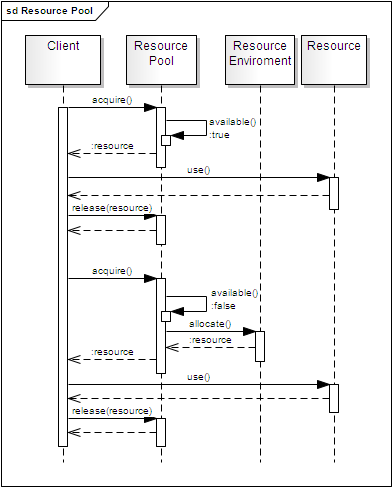
\includegraphics[width=7.75cm]{resource_pool}
\end{center}
\caption{Sequence diagram describing how acquisition and release of resources works in a system implementing the \emph{pooling pattern}: recycled objects are managed in a pool of resources, which allows pool clients to acquire them, and release them back to the pool when they are no longer needed.}
\label{fig:rp}
\end{figure}

To prevent the frequent acquisition and release of the aforementioned resources, our service makes use of the \emph{pooling pattern}~\citep{kircher2001}, in which multiple instances of one type of resource are managed in a pool. This pool of resources allows for reuse when resource clients release resources they no longer need: released resources are put back into the pool and made available to resource clients needing them, as shown in figure~\ref{fig:rp}.

To improve efficiency, the resource pool can eagerly acquire a number of resources after its creation; then, if demand exceeds the number of available resources in pool, more resources can be \emph{lazily} acquired.

There are various valid approaches to free unused resources, like those consisting of monitoring the use of a resource and controlling its lifecycle by using  strategies such as ``least recently used'' (LRU) or ``least frequently used'' (LFU), or introducing a \emph{lease} for every resource that specifies a time duration for which a resource can remain in the pool.

In our service, the default policy is to allocate new resources from the resource enviroment if there are no resources of the requested type available in the pool; the service also allows the setting of a \emph{high water mark}, i.e. a maximum number of allocated objects: if the number of allocated objects is equal to the high water mark, the requesting client has to wait in a queue until a resource of the requested type is available in the pool. In addition, as we made no prior assumptions about how the service would be used, it does not apply any garbage collection policy by default.

Relying on a resource pool is designed to result in the following improvements for our rule-based machine translation service:

\begin{description}
 \item[Performance] -- By preventing repetitious acquisition and release of resources;
 \item[Stability] -- Because repetitious acquisition and release of resource can increase the risk of system instability (for example, repetitious acquisition and release of memory can lead to fragmentation problems); %% SHOULD YOU PUT A REF HERE ? -FMT
%% If you want examples for "instability" (see comments by reviewer #2), then you can mention
%% that on at least one server using standard Apertium over a long-term period (one year), 
%% there have been numerous problems with run-away processes. For example:

%% http://bugs.apertium.org/cgi-bin/bugzilla/show_bug.cgi?id=37
%% http://bugs.apertium.org/cgi-bin/bugzilla/show_bug.cgi?id=31

%% and put (Tyers, p.c.); 
%% BEFORE you do this you should CHECK to see if the apertium-service would fix this. E.g. if 
%% lt-proc or apertium-tagger went awol, would the service kill them, or would it just bring
%% down the whole service ?

%% You can also mention security problems in scripts:
%%   http://bugs.apertium.org/cgi-bin/bugzilla/show_bug.cgi?id=76
%% Not that a service might not introduce new security problems!

 \item[Scalability] -- As resources can be used also in different types of translation tasks, avoiding the allocation of a complete set of resources for each different translation task (for example, translation tasks on different language pairs using different dictionaries can make use of the same resource for managing the removal and restoration of formatting).
\end{description}

\section{Results}

To evaluate the efficiency of our service, which we will refer to as {\tt apertium-service}, we compared the time it requires to compute and answer to a translation request from Spanish to English with the {\tt\small apertium-en-es} language pair\footnote{SVN Revision 16218} with the time required by the following systems:

%% REVIEWER #1: "I cannot see a reason for comparing the translation times for the 
%%      Apertium-based SOA system with those of a Moses SMT translator in the experiments. They 
%%      are completely heterogeneous machine translation systems and, most important, authors 
%%      are not responsible for the translation times. What does figure 3 show? The fact that 
%%      currently Apertium is faster than Moses is something we all know"

\begin{itemize}
 \item {\tt apertium}, a console application implemented as a part of the Apertium project;
% \item {\tt moses}~\citep{moses}, a Open Source Statistical Machine Translation system;
% \item {\tt moses-service}, a service relying on {\tt moses}.
\end{itemize}

%The translation model used by {\tt moses} and {\tt moses-service} has been trained on the well-known Europarl~\citep{europarl} corpus by using SRILM~\citep{srilm}, a toolkit for building and applying statistical language models. Language models have been then compiled into binary format using IRSTLM~\citep{irstlm}, and trained to minimize the error rate on a set of sentences from the same corpus. 
%
%\begin{figure}[!ht]
%\begin{center}
%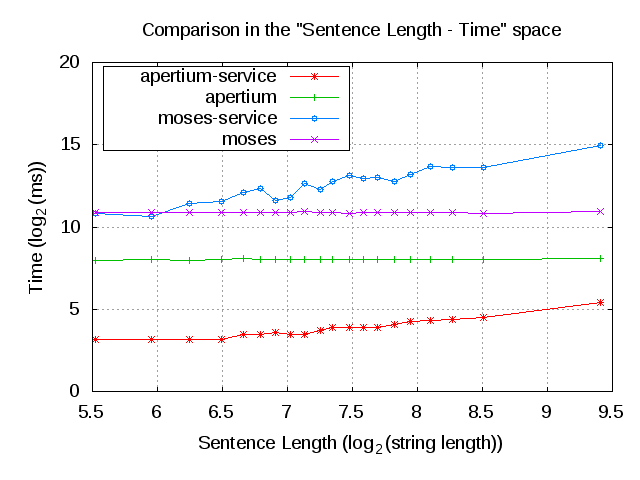
\includegraphics[width=7.75cm]{comp}
%\end{center}
%\caption{Comparison in the ``Sentence Length - Time'' space between {\tt apertium}, {\tt apertium-service}, {\tt moses} and {\tt moses-service}; measurements are in $log_{2}(string\ length)$ for the Sentence Length dimension and in $log_{2}(ms)$ for the Time dimension.}
%\label{fig:comp}
%\end{figure}
%
\begin{figure}[!ht]
\begin{center}
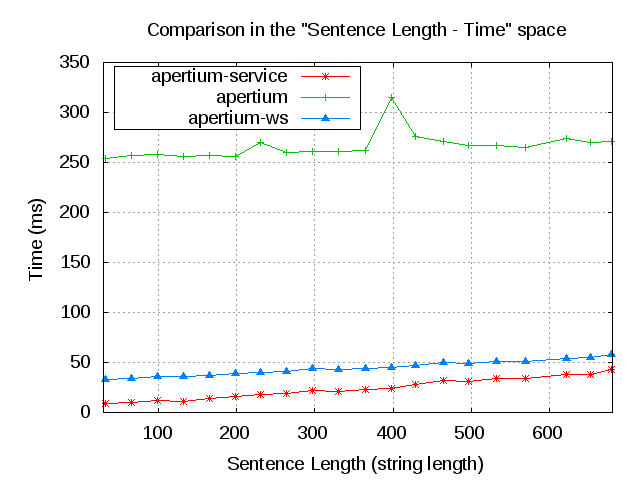
\includegraphics[width=7.75cm]{compap}
\end{center}
\caption{Comparison in the ``Sentence Length - Time'' space between {\tt apertium} and {\tt apertium-service}; measurements are in $string\ length$ for the Sentence Length dimension and in $ms$ for the Time dimension.}
\label{fig:compap}
\end{figure}

\begin{figure}[!ht]
\begin{center}
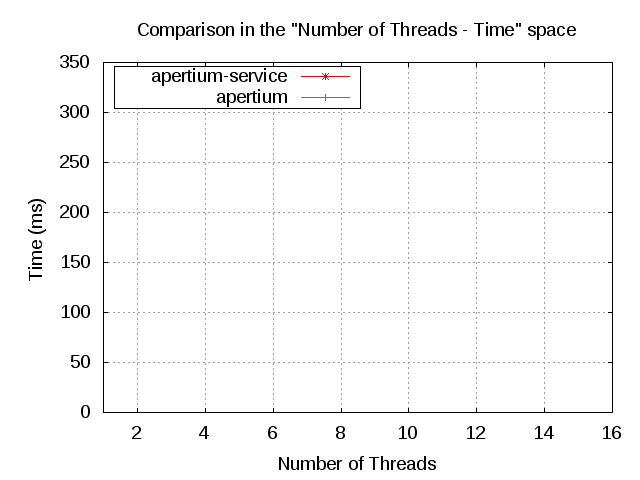
\includegraphics[width=7.75cm]{compmt}
\end{center}
\caption{Comparison in the ``Number of Threads- Time'' space between {\tt apertium} and {\tt apertium-service}.}
\label{fig:compmt}
\end{figure}

All the experiments were run on a server with four 2GHz Dual-Core AMD Opteron processors and 4GB of main memory, using the GNU/Linux operating system. Both {\tt\small apertium-service} and {\tt\small moses-service} were accepting translation requests in XML-RPC format, and the free text used for timing all the systems was also taken from Europarl corpus. Figure \ref{fig:comp} shows the time required to translate increasingly longer sentences for all systems (values in the time dimension are shown on a logarithmic scale), and figure~\ref{fig:compap} only for {\tt\small apertium-service} and {\tt\small apertium}.

Scalability for {\tt\small apertium} and {\tt\small apertium-service} have been evaluated by calculating the average time required by the two systems to answer to 1,024 translations requests sequentially sent by a variable number of clients; the requests consisted to translating the longest sentence from the Europarl evaluation corpus (679 characters) from Spanish to English. Figure \ref{fig:compmt} shows the results of this comparison.

%% Why did you choose the _longest_ sentence ? Wouldn't it have made sense to try different lengths of 
%% sentences ? If you did it so you could give a "worst case score" say so. -FMT


\section{Future work}

%% Here you should describe the case study, but in terms of future work. 

\paragraph{UMLS concept identification in non-English medical documents:} MetaMap~\citep{metamap} is an application that allows mapping text to UMLS Metathesaurus\footnote{The UMLS$^{\mbox{\small\textregistered}}$ Metathesaurus$^{\mbox{\small\textregistered}}$~\citep{umls} provides a representation of biomedical knowledge consisting of concepts classified by semantic type and both hierarchical and non-hierarchical relationships among the concepts.} concepts, which have proved to be useful for many applications, including decision support systems, management of patient records, information retrieval and data mining within the biomedical domain.

%% Fix this figure -- remake it in Graphviz or something -FMT
\begin{figure}[!ht]
\begin{center}
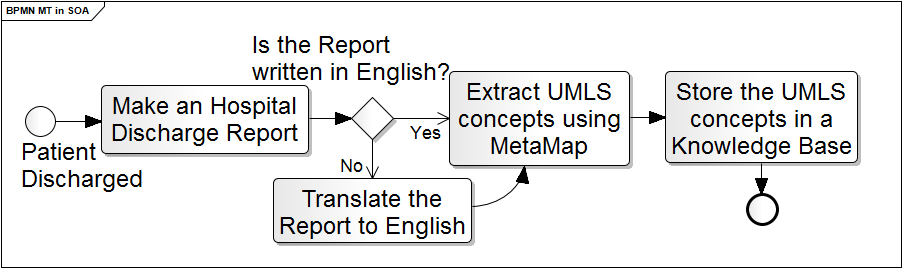
\includegraphics[width=7.75cm]{mtsoa}
\end{center}
\caption{Representation of a business process in which a clinical document, if written in a language different than English, is fist translated to English and then processed using MetaMap to extract UMLS concepts.}
\label{fig:mtsoa}
\end{figure}

Currently MetaMap is only available for English free text, which makes it difficult the use of UMLS Metathesaurus to represent concepts from biomedical texts written in languages other than English. A possible way to overcome this limitation consists in using machine translation specific for the biomedical domain to translate the free text from its original language to English, and then process it as in Figure \ref{fig:mtsoa}. This approach is discussed in \shortcite{metamapes}.

%
%\begin{cs}{\bf - Supporting creation of user-generated content:}
%Wikipedia is an online, multilingual, volunteer-edited encyclopedia. ``There are currently 262 language editions of Wikipedia; of these, 24 have over 100,000 articles and 81 have over 1,000 articles''~\citep{wikipedia}. Although access to technology is also an important factor, the number of available articles in a particular language's Wikipedia corresponds somewhat to the number of available speakers of that language.
%
%In many cases, closely related languages are mutually intelligible~\citep{tyers09a}, and even a prototype Machine Translation system can produce accurate translations~\citep{oller06}. This seems to be the case with Nynorsk and Bokmål~\citep{unhammer09}, where users of the Nynorsk Wikipedia have made contributions to the system's lexicon, to assist in their translation of articles from the larger Bokmål Wikipedia to the Nynorsk Wikipedia.
%
%However, the current use of Machine Translation on the Wikipedias of marginalized languages is a somewhat error-prone process, where the original text is manually copied from the source Wikipedia, translated off-line, and pasted as a new article to the target Wikipedia. By providing an efficient, easily integrated service, we hope to remove some of the accidental errors inherent to this process.
%
%In addition, the service's logging facilities may be used to improve Machine Translation quality, by incorporating user feedback~\citep{google}, in the form of corrections to the translated text. Small corrections to Wikipedia articles have been used in the construction of error corpora~\citep{milek08}, which can then be used to augment translation rules, or in the creation of statistical post-correction systems~\citep{dugast07}.
%\end{cs}
%


%% PUT THE METAMAP STUFF HERE -FMT


\section{Conclusions}

We presented {\tt\small apertium-service}, a machine translation service based on Apertium, a free/open-source rule-based machine translation platform. It has been shown to be competitive compared to the baseline system in both efficiency and scalability.

Source code for our service is released under the GNU General Public Licence version 3\footnote{\url{http://www.gnu.org/licenses/gpl.html}} and is available on the Apertium SVN repository.\footnote{{\small\url{http://apertium.svn.sourceforge.net/svnroot/apertium/trunk/apertium-service}}}

\section*{Acknowledgements}

Development for this project was funded as part of the Google Summer of Code\footnote{\url{http://code.google.com/soc/}} programme.
Many thanks go to Jimmy O'Regan, Francis Tyers and others involved in the Apertium Project, for their constant help. Additionally I am grateful to the anonymous reviewers for their invaluable comments and suggestions on an earlier version of this paper.

\bibliographystyle{apalike}
\bibliography{freerbmt09}

\end{document}
